\subsection{实验目的}
掌握一些基本的图像融合方法,包括基于像素灰度值的简单图像融合算法,以及彩色图像的分解于合成。完成遥感图像的图像融合。
\subsection{实验原理}
\subsubsection{图像融合的概念}
综合和提取两个或多个圆的图像信息,获得对同一场景或者目标更为准确、全面、可靠的图像,使之更适合人眼感知或计算机后续处理。
\begin{figure}[H]
	\centering
	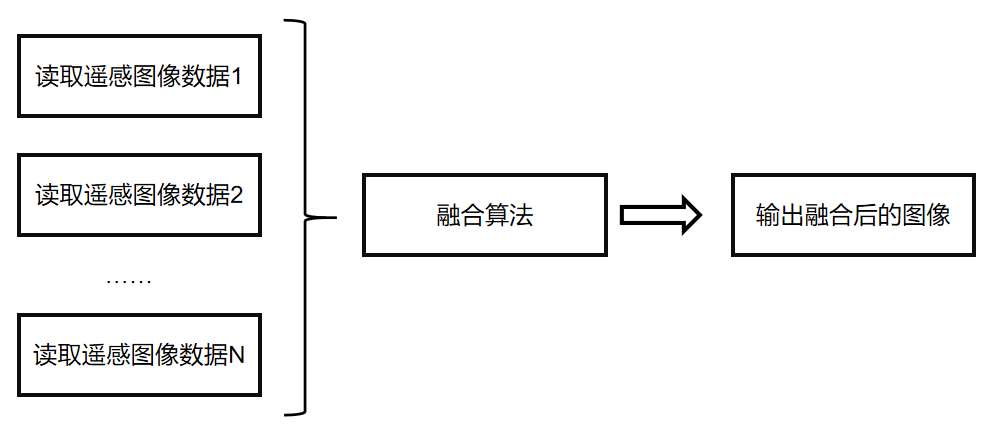
\includegraphics[width=0.7\linewidth]{figure/fusion_flowchart.png}
	\caption{图像融合算法流程图}
	\label{fig:fusion_flowchart}
\end{figure}
\subsubsection{简单的图像融合算法}
\begin{description}
	\item[像素灰度值平均或加权平均法]
	\[ I(x, y)=\frac{\sum_{n=1}^{N}W^n(x, y)I^n(x, y)}{\sum_{n=1}^{N}W^n(x, y)} \]
	\[ W^n(x, y)=\frac{1}{N} \]
	\item[像素灰度值选大法] 
	\[ I(x, y)=\max_n\{I^n(x, y),\quad n=1,2,\dots N\} \]
	\item[像素灰度值选小法] 
	\[ I(x, y)=\min_n\{I^n(x, y),\quad 1,2,\dots N\} \]
\end{description}
\subsubsection{彩色图像的分解与合成}
\begin{description}
	\item[能量图像] 
	\[ I=Ir+Ig+Ib \]
	\item[变换后的彩色图像合成]
	蓝色分量:加高斯噪声污染
	
	绿色分量:进行对数变换
	
	红色分量:进行图像反转
	
	重新合成彩色图像
\end{description}
\subsubsection{彩色图像合成}
通过图像变换与融合突出图像中感兴趣的目标。
\subsubsection{通过图像融合得到变化检测差异图}
\begin{description}
	\item[差异图像] 
	\[ I1=1-\min \left( \frac{\mu_1}{\mu_2},\frac{\mu_2}{\mu_1} \right)  \]
	\[ I2= \left| \log\frac{X_2}{X_1} \right| = \left| \log X_2 - \log X_1 \right|  \]
	\item[图像融合]
	两个差异图的低频成分平均融合,高频成分取小融合。
\end{description}
\subsection{实验流程}
\begin{figure}[H]
	\centering
	\begin{tikzpicture}[node distance=1.5cm]
	\node(start) [startstop] {开始};
	\node(inputimg) [io, below of=start] {读取图片};
	\node(separateimg) [process, below of=inputimg] {分离彩色图像颜色通道};
	\node(fusionchannels) [process, below of=separateimg] {加权合并各通道能量};
	\node(outputenergyimg) [io, below of=fusionchannels] {输出能量合成图像};
	\node(channelcompare) [process, below of=outputenergyimg] {使用图片的两个不同通道进行对比};
	\node(outputchannelcomparation) [io, below of=channelcompare] {输出比较的结果};
	\node(channeltransform) [process, below of=outputchannelcomparation] {对各个通道分别进行变换};
	\node(outputtransformed) [io, below of=channeltransform] {输出变换后的图像};
	\node(inputmask) [io, below of=outputtransformed] {输入兴趣区域蒙版};
	\node(interestedarea) [process, below of=inputmask] {合成兴趣区域图像};
	\node(outputinterestedarea) [io, below of=interestedarea] {输出兴趣区域图像};
	\node(end) [startstop, below of=outputinterestedarea] {结束};
	
	\draw[arrow] (start) -- (inputimg);
	\draw[arrow] (inputimg) -- (separateimg);
	\draw[arrow] (separateimg) -- (fusionchannels);
	\draw[arrow] (fusionchannels) -- (outputenergyimg);
	\draw[arrow] (outputenergyimg) -- (channelcompare);
	\draw[arrow] (channelcompare) -- (outputchannelcomparation);
	\draw[arrow] (outputchannelcomparation) -- (channeltransform);
	\draw[arrow] (channeltransform) -- (outputtransformed);
	\draw[arrow] (outputtransformed) -- (inputmask);
	\draw[arrow] (inputmask) -- (interestedarea);
	\draw[arrow] (interestedarea) -- (outputinterestedarea);
	\draw[arrow] (outputinterestedarea) -- (end);
	\end{tikzpicture}
\end{figure}
\subsection{实验程序}
\lstinputlisting[caption={生成彩色图像的能量图像程序}]{"../Executable Script/Exp 3/ColorImageEnergyGraph.m"}
\lstinputlisting[caption={彩色图像的分解变换与合成程序}]{"../Executable Script/Exp 3/ColorImageTransformAndFusion.m"}
\lstinputlisting[caption={生成彩色图像的通道差异程序}]{"../Executable Script/Exp 3/ColorImageChannelsDiffer.m"}
\lstinputlisting[caption={$I_1=1-\min\left(\frac{\mu_1}{\mu_2},\frac{\mu_2}{\mu_1} \right) $差异图像生成函数}]{"../Function Library/ImageDiffer_Minus.m"}
\lstinputlisting[caption={$I_1=\left|\log X_1-\log X_2 \right| $差异图像生成函数}]{"../Function Library/ImageDiffer_Log.m"}
\lstinputlisting[caption={差异图像融合函数}]{"../Function Library/ImageDiffer.m"}
\lstinputlisting[caption={在图中标记兴趣区域程序}]{"../Executable Script/Exp 3/MarkInterestArea.m"}
\lstinputlisting[caption={图像加权融合函数}]{"../Function Library/SafetyConstantImageMultiply.m"}
\subsection{实验结果和分析}
\subsubsection{生成彩色图像的能量图像}
对原图片的红色、绿色和蓝色通道按照1、1、1的权重进行加权融合并重新进行量化,即可得到融合了红绿蓝三通道能量的能量图像,如图\ref{fig:dji0027energy}所示。
\begin{figure}[H]
	\centering	
	\begin{minipage}{0.45\linewidth}
		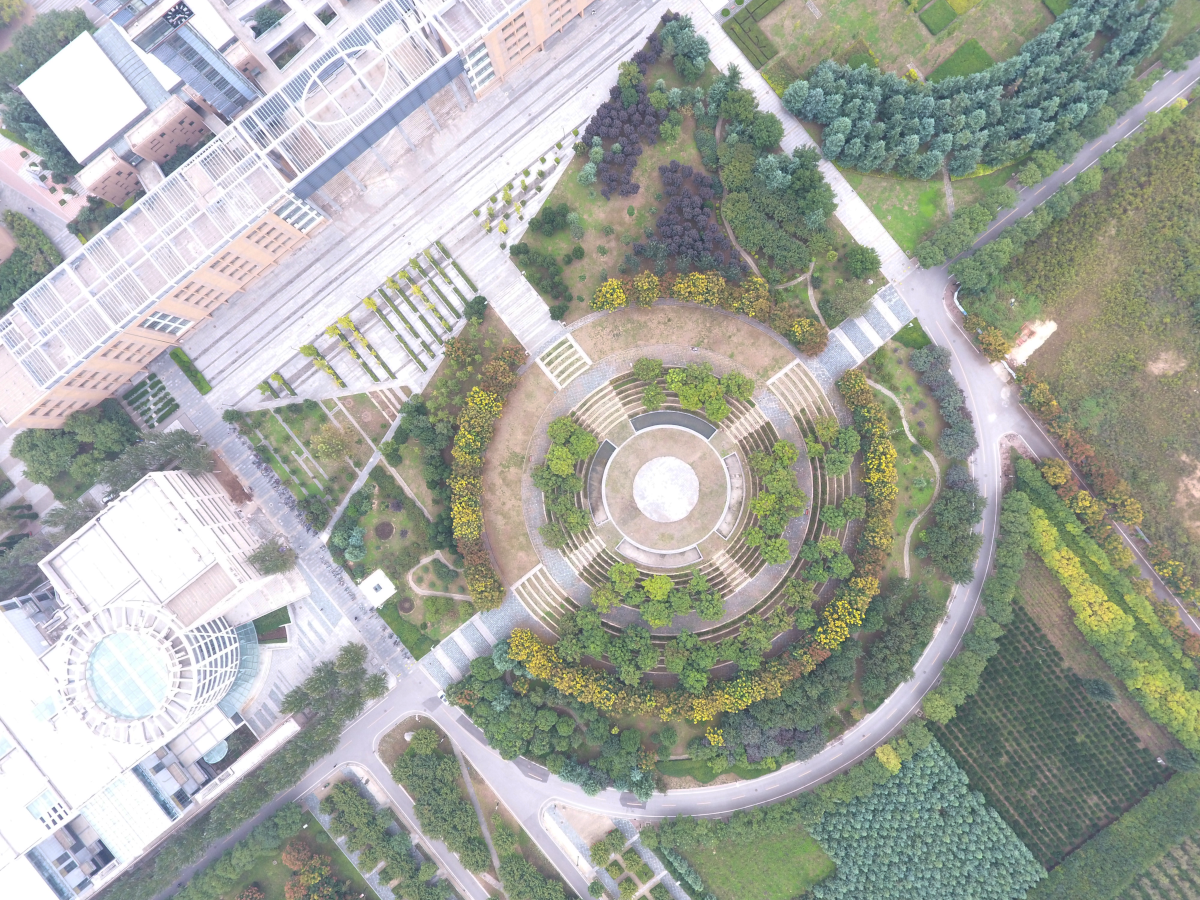
\includegraphics[width=\linewidth]{figure/DJI_0027_Compressed.png}
		\caption{原图片}
		\label{fig:dji0027original}
	\end{minipage}
	\begin{minipage}{0.45\linewidth}
		\includegraphics[width=\linewidth]{figure/DJI_0027_Energy.png}
		\caption{彩色图像的能量图像}
		\label{fig:dji0027energy}
	\end{minipage}
\end{figure}
\subsubsection{彩色图像的分解变换与合成}
对如图\ref{fig:dji0027original}所示的原图像进行红、绿、蓝通道进行分解,并且对红色分量增加高斯白噪声,对绿色分量进行$s=\log_{1.2}(1+0.2r)$的对数变换,对蓝色分量进行反转变换,可以得到如图\ref{fig:dji0027color_transform_fusion}所示的结果。
\begin{figure}[H]
	\centering
	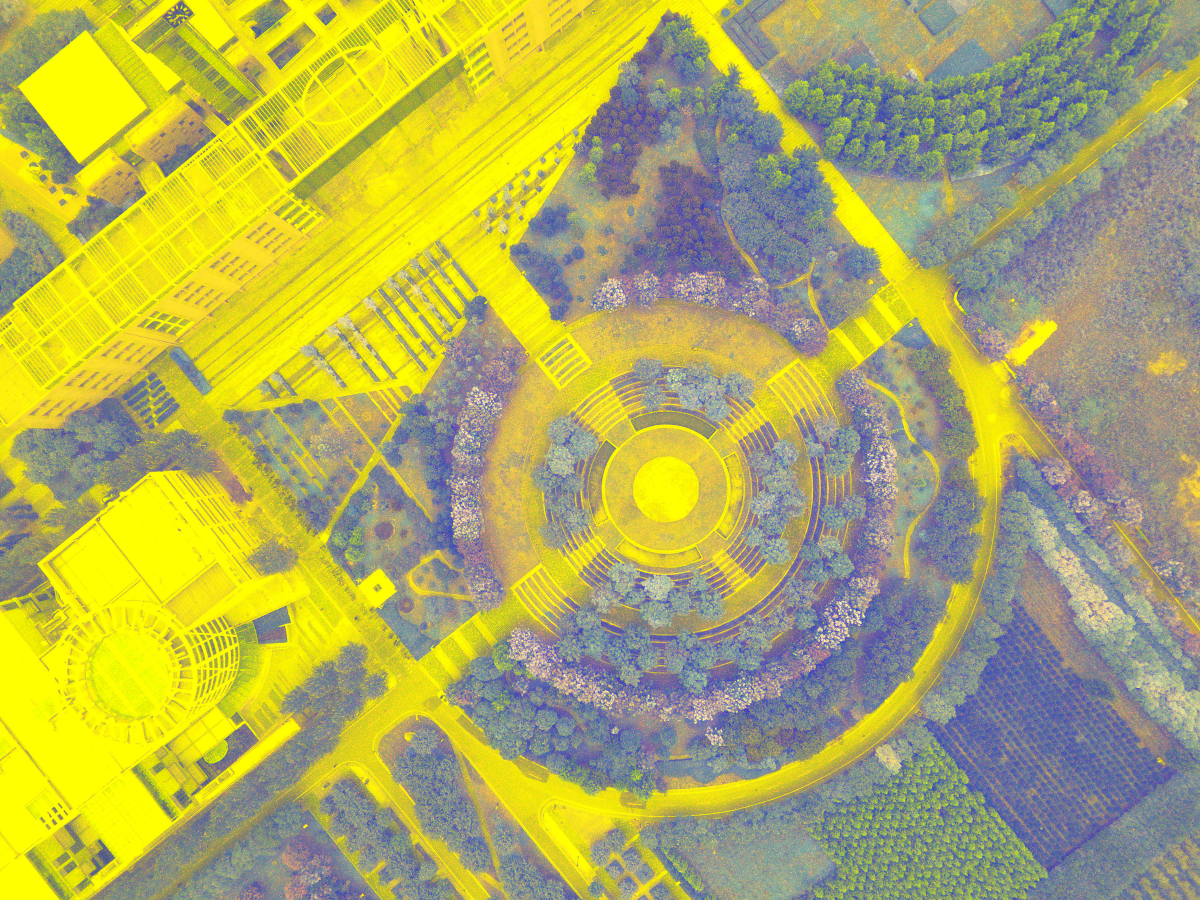
\includegraphics[width=0.7\linewidth]{figure/DJI_0027_Transformed_Fusion.png}
	\caption{彩色图像的分解变换与合成结果}
	\label{fig:dji0027color_transform_fusion}
\end{figure}
\subsubsection{彩色图像两通道图像差异}
\begin{figure}[H]
	\centering
	\begin{minipage}{0.45\linewidth}
		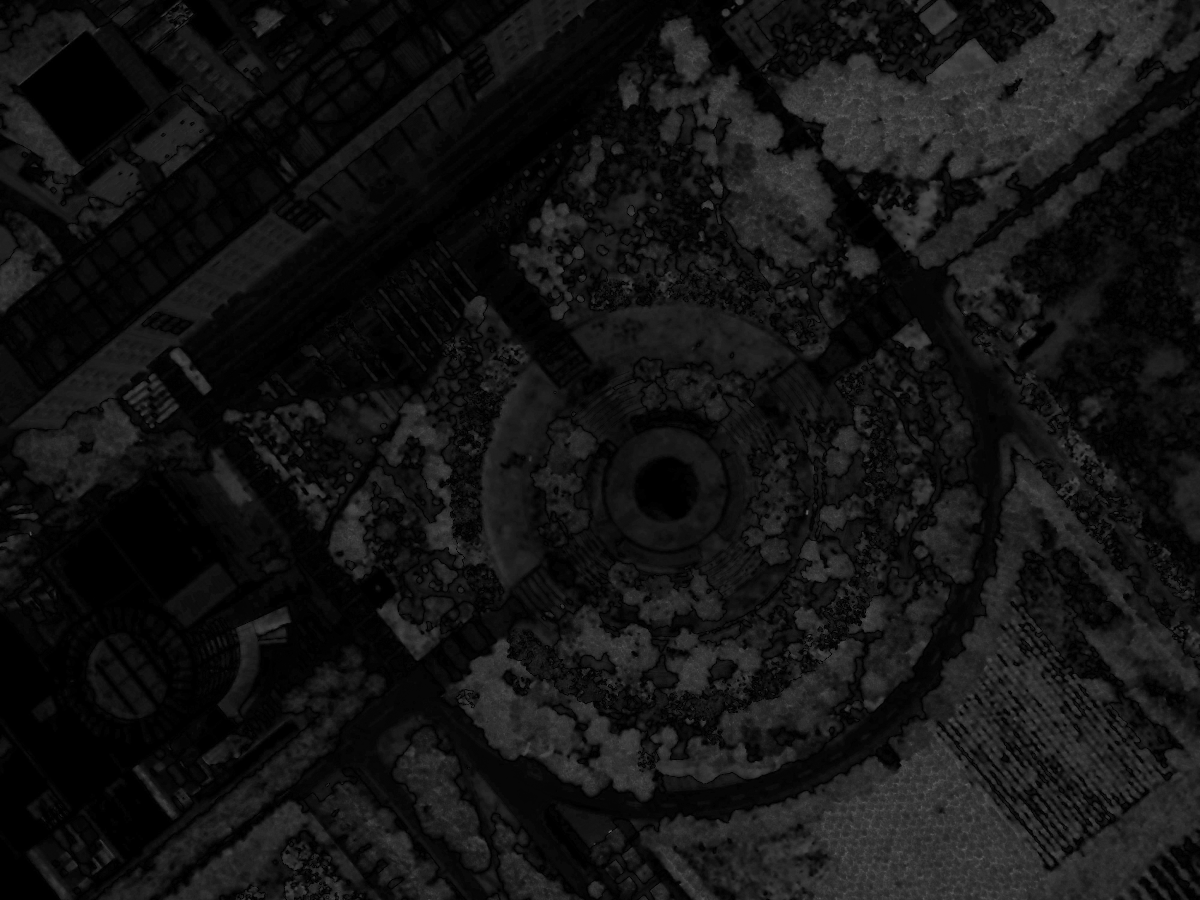
\includegraphics[width=\linewidth]{figure/DJI_0027_Minus_Differ.png}
		\caption{采用$I_1=1-\min\left(\frac{\mu_1}{\mu_2},\frac{\mu_2}{\mu_1} \right) $计算差异图像的结果}
	\end{minipage}
	\begin{minipage}{0.45\linewidth}
		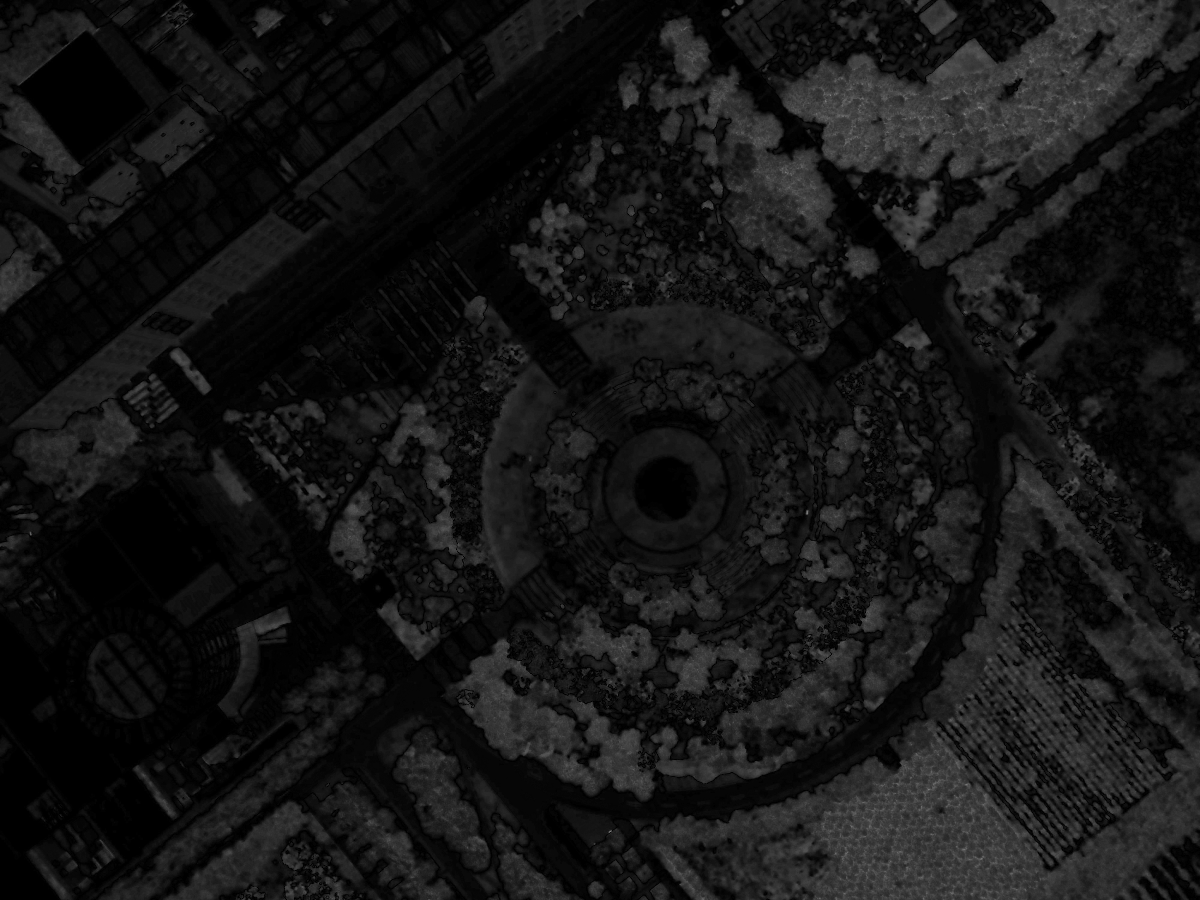
\includegraphics[width=\linewidth]{figure/DJI_0027_Log_Differ.png}
		\caption{采用$I_1=\left|\log X_1-\log X_2 \right| $计算差异图像的结果}
	\end{minipage}
\end{figure}
\subsubsection{差异图像的融合}
对以上两幅差异图像进行融合,可以得到如图\ref{fig:dji0027differ}所示的融合的差异图像。
\begin{figure}[H]
	\centering
	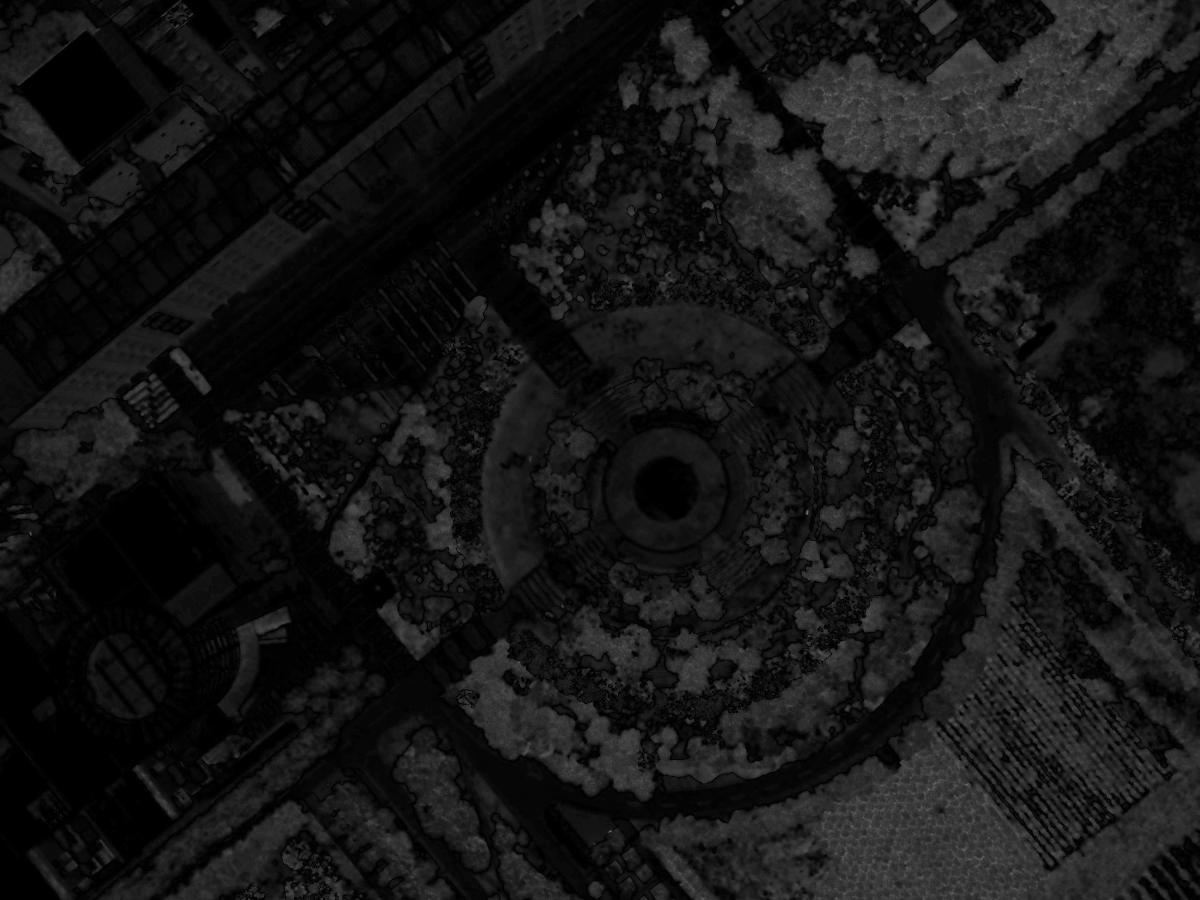
\includegraphics[width=0.7\linewidth]{figure/DJI_0027_Differ.png}
	\caption{差异图像的融合图像}
	\label{fig:dji0027differ}
\end{figure}
\subsubsection{标记兴趣区域}
假设我们对图片中的图书馆感兴趣,将图书馆设为兴趣区域,在对应的二值蒙版中将图书馆所在区域设置为“1”,其他部分设置为“0”。对图书馆所在的区域和其他区域进行不同的变换,再进行图像融合,即可突出图书馆在图片中的区域。
\begin{figure}[H]
	\centering
	\begin{minipage}{0.45\linewidth}
		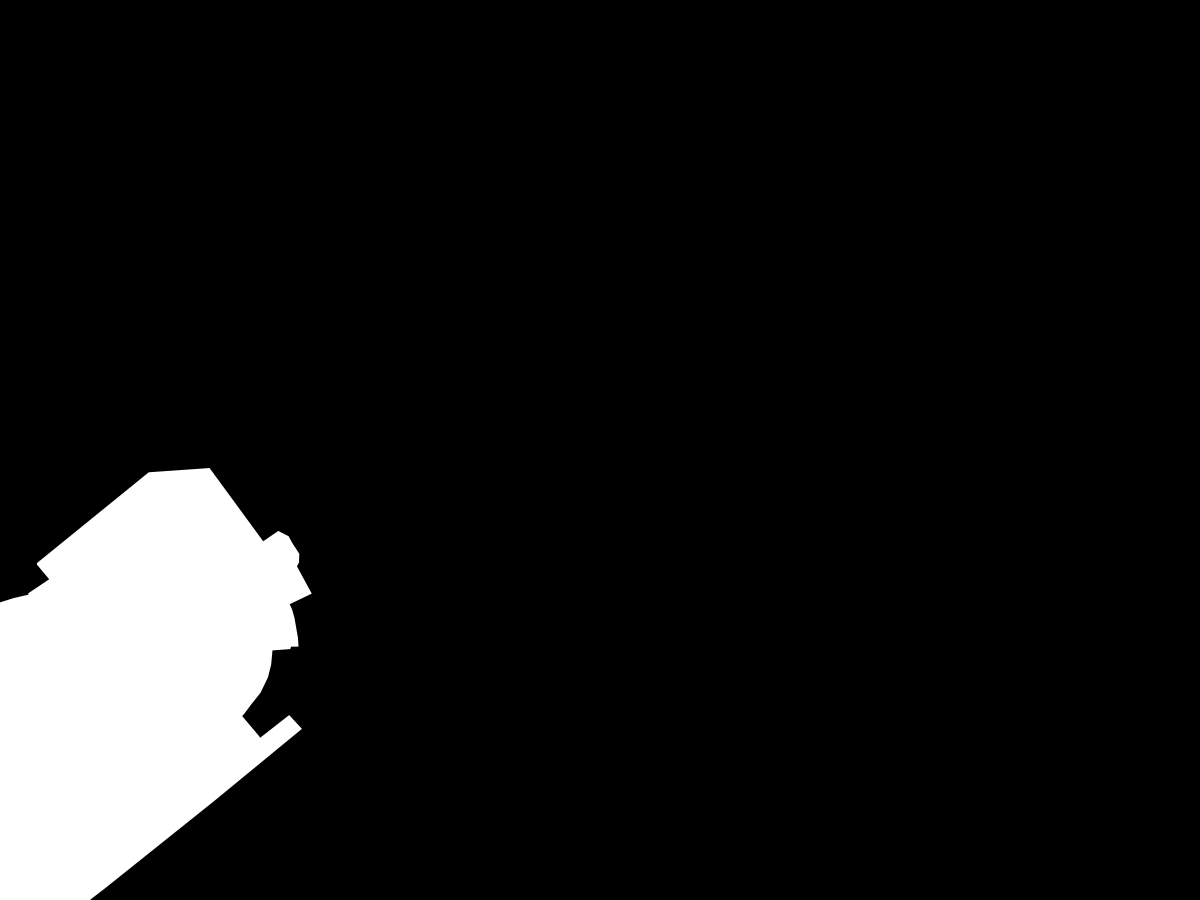
\includegraphics[width=\linewidth]{figure/DJI_0027_Compressed_Mask.png}
		\caption{用于标记兴趣区域的二值蒙版}
	\end{minipage}
	\begin{minipage}{0.45\linewidth}
		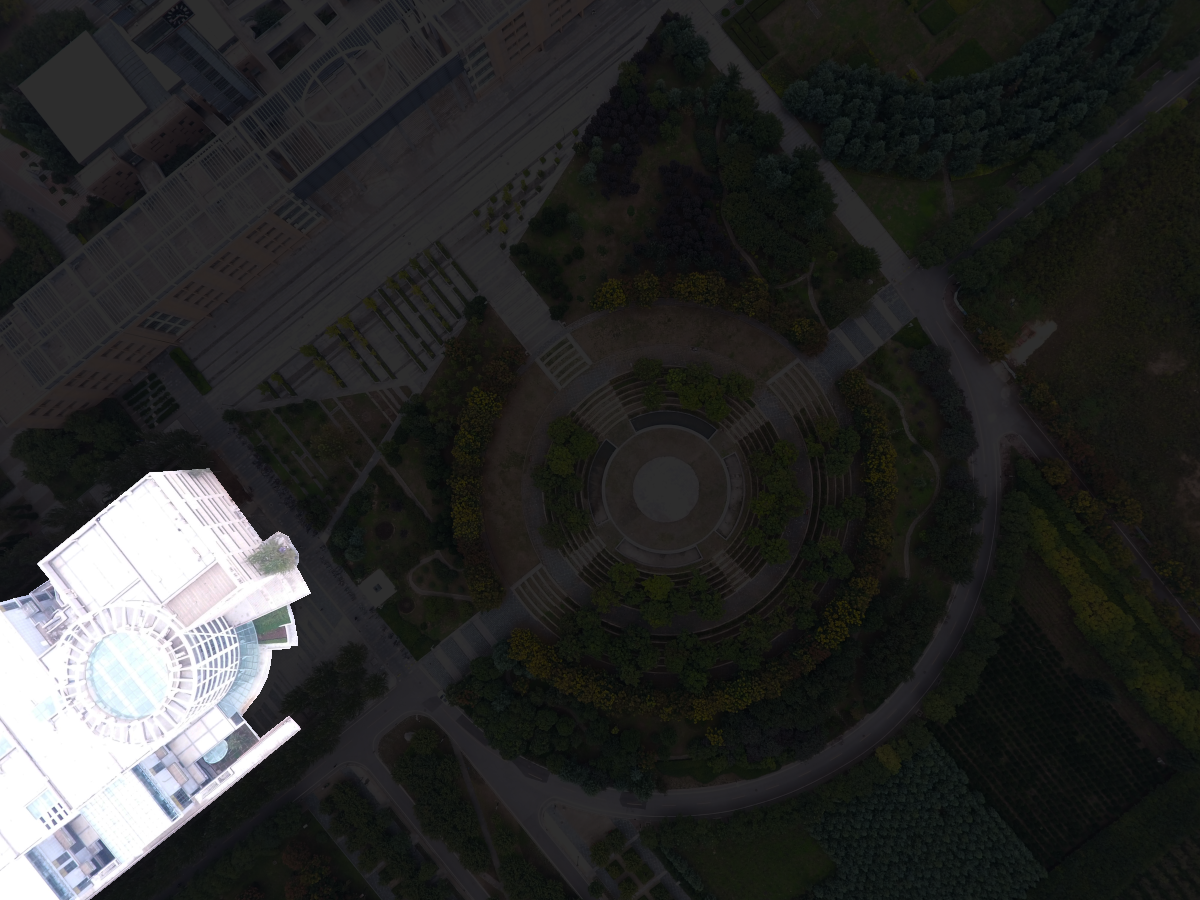
\includegraphics[width=\linewidth]{figure/DJI_0027_Interest.png}
		\caption{突出兴趣区域的图像}
	\end{minipage}
\end{figure}
使用简单的灰度值平均或加权平均法融合的图像更符合人眼的直觉。简单的灰度值平均或加权平均法能够实现对不同区域和图像的明暗变化,能够更好地突出对不同区域亮度值的选择与区分。

使用简单的灰度值平均或加权平均法融合的图像可以控制要突出显示的目标轮廓、位置和纹理特征,适合小局部的目标辨别。差异图像的融合能够迅速地对全图的差异进行处理,适合大范围、零碎、没有明确边界特征和位置特征的目标的判断与识别,适合用于统计分析。